%%%%%%%%%%%%%%%%%%%%%%%%%%%%%%%%%%%%%%%%%%%%%%%%%%%%%%%%%%%%%%%%%%%%%%%%%%%%
%% Trim Size: 9.75in x 6.5in
%% Text Area: 8in (include Runningheads) x 5in
%% ws-ijufks.tex   :   25-9-06
%% Tex file to use with ws-ijufks.cls written in Latex2E. 
%% The content, structure, format and layout of this style file is the 
%% property of World Scientific Publishing Co. Pte. Ltd. 
%% Copyright 1995, 2002 by World Scientific Publishing Co. 
%% All rights are reserved.
%%%%%%%%%%%%%%%%%%%%%%%%%%%%%%%%%%%%%%%%%%%%%%%%%%%%%%%%%%%%%%%%%%%%%%%%%%%%

%

\documentclass{ws-ijufks}
%\usepackage{titlesec}
%\setcounter{secnumdepth}{4}
\usepackage{graphicx}
%\usepackage{amsthm}
\usepackage{amssymb}
\usepackage{mathtools}
\usepackage{booktabs} %For position cell elements in Tables %
\usepackage{array}
\usepackage{multirow} %for MULTIROW Tables %
%\usepackage{enumerate}
\usepackage{placeins}
\usepackage{varwidth}
\usepackage{soul}
\usepackage{undertilde}
\usepackage{algorithm}
\usepackage{algpseudocode}
\graphicspath{{Images/}}

\begin{document}

%\markboth{G. S. M. Thakur, R. Bhattacharyya, S. S. Mondal}
%{Fuzzy ES for Portfolio Selection}

%%%%%%%%%%%%%%%%%%%%% Publisher's Area please ignore %%%%%%%%%%%%%%%
%
%\catchline{}{}{}{}{}
%
%%%%%%%%%%%%%%%%%%%%%%%%%%%%%%%%%%%%%%%%%%%%%%%%%%%%%%%%%%%%%%%%%%%%

\title{FUZZY EXPERT SYSTEM FOR STOCK PORTFOLIO SELECTION: AN APPLICATION TO BOMBAY STOCK EXCHANGE} 
%\LaTeX\footnote{Typeset title in 10 pt Times Roman uppercase and boldface. Please write down in 
%pencil a short title to be used as the running head.}}

\author{GOUR SUNDAR MITRA THAKUR}

%\footnote{Typeset names in 8 pt Times Roman,
%uppercase and lightface. Use footnotes only to indicate if
%permanent and present addresses are different. Funding
%information should go in the Acknowledgements section.}}

\address{Department of Computer Science and Engineering,\\ Dr. B. C. Roy Engg. College, Durgapur, West Bengal, India\\
	cse.gsmt@gmail.com}
%\footnote{State completely without abbreviations, the 
%affiliation and mailing address, including country. Typeset in 
%8~pt Times italic.}\\


\author{RUPAK BHATTACHARYYA}

\address{Department of Mathematics,\\ Bijoy Krishna Girls' College, Howrah, West Bengal, India\\
mathsrup@gmail.com}

\author{SEEMA SARKAR MONDAL}

\address{Department of Mathematics\\ National Institute of Technology Durgapur, West Bengal, India\\
	seemasarkarmondal@yahoo.co.in}

\maketitle

%\begin{history}
%\received{(received date)}
%\revised{(revised date)}
%%\accepted{(Day Month Year)}
%%\comby{(xxxxxxxxxx)}
%\end{history}

\begin{abstract}
Selection of proper stocks, before allocating investment ratios, is always a crucial task for the investors. Presence 
of many influencing factors in stock performance have motivated researchers to adopt various Artificial Intelligence 
(AI) techniques to make this challenging task easier. In this paper a novel fuzzy expert system model is proposed to 
evaluate and rank the stocks under Bombay Stock Exchange (BSE). Fuzzy Delphi method is used to identify the critical 
factors initially and then factors with lower correlation coefficients are finally considered for further 
consideration. Dempster-Shafer (DS) evidence theory is used for the first time to automatically generate the 
consequents of the fuzzy rule base to reduce the effort in knowledge base development of the expert system. Later a 
portfolio optimization model is constructed where the objective function is considered as the ratio of the difference 
of fuzzy portfolio return and the risk free return to the weighted mean semi-variance of the assets that has been used. 
The model is solved by applying Ant Colony Optimization (ACO) algorithm by giving preference to the top ranked stocks. 
The performance of the model proved to be satisfactory for short-term investment period when compared with the recent 
performance of the stocks. The model is also proved to be more efficient and robust when compared with other existing 
expert system models for stock selection and portfolio recommendation. 
\end{abstract}

\keywords{Ranking of stocks; Stock Portfolio Selection; Fuzzy rule-based system; Dempster-Shafer Theory; Fuzzy Delphi 
method.}

\section{Introduction}	
Stock portfolio selection is basically an optimal allocation of investor' assets among 
certain number of stocks to provide maximum return with minimum risk. There are different 
types of factors which directly or indirectly influence the performance of stocks. This 
makes the task of stock selection and portfolio construction challenging and uncertain 
for the stock market researchers since the beginning. According to the work of Markowitz 
\cite{Markowitz1952} portfolio selection may include two stages: firstly, performances of 
different securities is observed with beliefs about their future performances and 
secondly, a proper choice of portfolio is made with relevant beliefs about future 
performances. The main aim in Modern Portfolio Theory (MPT) of investment is to maximize 
the expected return of the portfolio for a given amount of portfolio risk or  
equivalently  minimize risk for a given level of expected return, by carefully choosing 
the proportions of various assets. In the ground-breaking work, Markowitz 
\cite{Markowitz1952} has quantified return as the mean and variance as the risk of the 
portfolio of securities. The relationship between risk and mean-variance are later 
examined in various researches \cite{Zhou2000,Fang2006,Ogryczak2000,Huang2008}. The twin 
objectives of investors', profit maximization and risk minimization, are thus quantified.

Portfolio selection problem is proved to be a multi-dimensional problem and to solve this 
inherent multi-criteria nature of this problem Multi-criteria Decision Making (MCDM) 
approach is adopted in various researches like 
\cite{Xidonas2011,Edwards2007,Abdollahzadeh2002,Siskos1989}. In spite of all these 
efforts researchers were facing difficulties in bringing efficiency in portfolios 
specially in dynamic uncertain environment. As a result the use of different AI 
techniques in stock selection and portfolio construction became inevitable due to their 
well known capability of handling uncertain and vague data. In this article a DS theory 
based fuzzy expert system model is proposed. 

The rest of the paper is organized as follows: section 2 gives a brief literature review 
where some significant researches, applying different AI and soft computing techniques in 
stock selection and portfolio recommendation, are introduced. In section 3 the proposed 
approach and its application is demonstrated. Selection of four critical factors and 
their importance in stock performance are discussed in section 4. In section 5 the 
concepts DS evidence theory and fuzzy expert system are briefly discussed. In section 6 
the process of collecting historical data from BSE and its fuzzification process is 
explained. Fuzzy rule construction using DS theory is elaborated in section 7. In section 
8 ranking of of stocks under BSE are demonstrated. Portfolio optimization process is 
elaborated in section 9. Results of the proposed model are analyzed and compared in 
section 10. Finally section 11 gives the conclusion.

\section{Literature Review}
In literature we can find wide use of different AI and Soft Computing techniques to 
analyse and predict the performance of stocks in various stock exchanges around the 
world. In some researches 
\cite{Adebiyi2012ANN,Fernandez2007ANN,Ko2008ANN,Olatunji2011ANN,De2011ANN} efficient 
learning capability of Artificial Neural Network (ANN) is adopted to select stocks and 
construct portfolios whereas in some other researches 
\cite{Chen2009GAa,Chang2009GA,Chen2009GAb,Jiao2007GA,Chen2010GA} optimization capability 
of Genetic Algorithm is used for portfolio optimization. But the application of Fuzzy 
Logic and Fuzzy Set theory has become the most popular among other soft computing 
techniques, due to its uncertainty handling capability and the efficiency to 
incorporate vagueness in investors' preferences in portfolio construction. 

In a research \cite{Tiryaki2005fuzzy} proposed a new method regarding fuzzy MCDM 
by making some modification of Chen's Method \cite{chen2001fuzzy} and applied it to the 
stocks selection on Istanbul Stock Exchange (ISE). In another article 
\cite{Bilbao2006fuzzy} applied fuzzy set theory to the problem of portfolio selection 
using Sharpe’s single-index model as a basis. In another article a portfolio rank-index 
is proposed by \cite{Bermudez2007fuzzy} that allows us to rank a finite set of 
portfolios based on the well-known value-ambiguity indices of trapezoidal fuzzy numbers. 
In another research \cite{Fasanghari2010design} described a new method for design of 
fuzzy expert system for portfolio recommendation at Taiwan stock exchange (TSE).

\section{Proposed Approach and its Application}

Portfolio selection process can be divided into two stages \cite{Xidonas2009}. In the first stage, some stocks are 
selected to construct the portfolio and in the second stage, the percentage of the total value for each stock is 
identified. Use of fuzzy expert systems in the selection of stocks and equity have recently become very effective and 
popular. In a work Fasanghari et al. \cite{Fasanghari2010design} developed an fuzzy expert system to select superior 
stocks in Tehran Stock Exchange (TSE) by identifying $7$ factors influencing the stock market. A rule base of total 932 
rules was constructed for this purpose. Though no proper portfolio optimization model was used in this work, the 
outcome of the model proved to be satisfactory. But the major concern of this model can be the development time and 
cost due to repetitive expert interactions for the development of the model. Authors have used only fuzzy set theory to 
deal with the inherent uncertainty present in the rule base though fuzzy set theory is more effective in dealing with 
vagueness in the model than addressing inherent uncertainty of the model \cite{Rodriguez2012hesitant}. In another 
significant work Xidonas et al.\cite{Xidonas2009} developed an expert system for the selection of equity securities but 
the concerns remained more or less same as the previous one.

In this research selection of stocks are made with the help of an expert system where the fuzzy rule base is 
automatically generated by applying DS evidence theory. 
\begin{itemize}
	\item This has minimized the overall development time and cost as the required number of expert interactions is 
	reduced considerably.
	\item  DS evidence	theory is well known for its capability of dealing with incomplete and uncertain information. 
	So another level of	uncertainty handling mechanism beside fuzzy set theory is incorporated in the model.
\end{itemize}
The proposed model is implemented in two phases.

\begin{enumerate}
\item Initially $10$ investment ratios are selected as critical factors. Then the number of factors are reduced to $6$ 
by applying fuzzy Delphi method. After calculating correlation coefficients among these factors, $4$ factors with 
minimum correlations are finally selected and their historical data for the period of FY 
2003-04 to FY 2012-13 are collected. These four factors have functioned as the input of 
the proposed DS fuzzy expert system and their historical data have been used to generate 
the consequents of the fuzzy rules with the help of DS evidence theory. The 
model is tested with the historical data of FY 2012-13, when values of these four factors 
for each stocks are provided as input to the fuzzy inference system and then they are 
ranked based on their defuzzified output.
\item A portfolio optimization model is constructed and then it is solved with ACO by 
considering top 10 stocks, as per the previous ranking, in the portfolio, to allocate 
investment ratios by giving preferences to the top ranked stocks.	 
\end{enumerate}
The model is tested with the data of FY 2012-13 to predict the performance of different 
stocks in FY 2013-14, FY 2014-15 and FY 2015-16. Performance of the model is proved to be 
satisfactory when compared with the actual performance of stocks.
Figure \ref{fig:F1} depicts the brief structure of the article.
\begin{figure}[h]
	\centering
	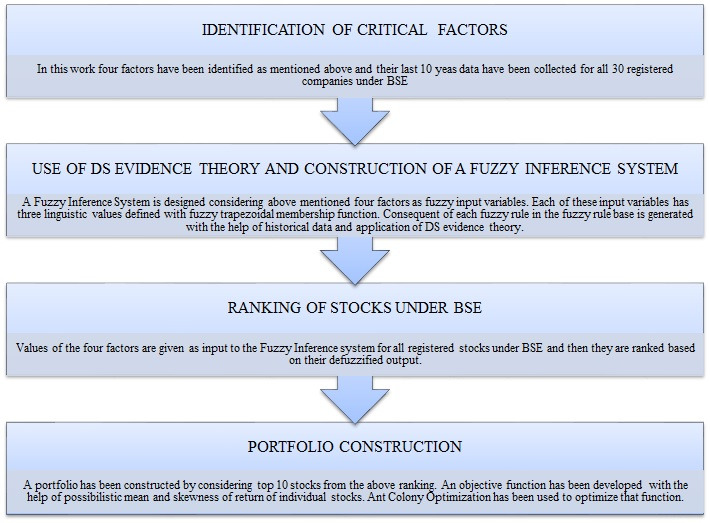
\includegraphics[width=8cm,height=7cm]{article_structure}
	\caption{Design diagram of the proposed inflation forecasting model}
	\label{fig:F1}
\end{figure} 

\section{Identification of Critical Factors}
According to value investors, there is no \emph{right way} to analyze stocks due to the presence of multi-dimensional 
uncertainties. Stock market experts in BSE use many factors for the evaluation and selection of stocks. With the help 
of various experts' opinions and thorough literature survey, initially following 10 
metrics (ratios) are identified.

\subsection*{Price to earnings (P/E)}
The price to earnings ratio (P/E) is a valuation ratio of a stock that is determined by 
market value per share divided by earnings per share (EPS) of the stock.
\begin{equation*}
\frac{P}{E}=\frac{\textrm{Market value per share}}{EPS}
\end{equation*}
In general, a high price to earnings ratio for any company indicates that investors are 
expecting higher earnings growth in future from it compared to companies with a lower 
price to earnings ratio.

\subsection*{Payout ratio}
The payout ratio can be expressed as dividends paid out as a proportion of cash flow. It 
can also be expressed as the proportion of earnings paid out as dividends to 
shareholders, typically expressed as percentage.

\begin{equation*}
Payout ratio=\frac{\textrm{Total dividends paid}}{\textrm{Net income}} \times 100
\end{equation*}

\subsection*{Earning per share(EPS)}
It is the portion of a company's profit allocated to each outstanding share of common 
stock. Earning per share serves as indicator of a company's profitability and it is 
calculated as:
\begin{equation*}
EPS=\frac{\text{\emph{Net income}}-\text{\emph{Dividends on preferred 
stock}}}{\text{\emph{Average outstanding of 
			shares}}}
\end{equation*} 

\subsection*{Price-to-book value (P/B)}
Price-to-book vale (P/B) is the ratio of market value of a company's shares over its book 
value of equity.
\begin{equation*}
\frac{P}{B}=\frac{\textrm{Stock price}}{\textrm{Total asset}-\textrm{Liabilities}}
\end{equation*}
\subsection*{Price to sales (P/S)}

The price to sales ratio is another valuation ratio that compares a company's stock price 
to its revenues. It can be calculated by dividing the company's market capitalization by 
its total sale. This ratio is also known as revenue multiple or sales multiple.
\begin{equation*}
\frac{P}{S}=\frac{\textrm{Market Capitalization}}{\textrm{Total Sales}}
\end{equation*}

\subsection*{Long term debt/equity (LTDER):}
The long term debt to equity ratio is the ratio of total liabilities of a stock to its 
shareholders' equity. It is a leverage ratio and it measures the degree to which the 
assets of the stock are financed by the debts and the shareholders' equity of a stock.  
It is calculated by the total liabilities divided by shareholders' equity.

\begin{equation*}
LTDER=\frac{\textrm{Total Liabilities}}{\textrm{Shareholders' Equity}}
\end{equation*}

\subsection*{Price-to-cash-flow ratio (P/CF)}
The price-to-cash-flow ratio is a stock valuation indicator that measures the value of a 
stock's price to its cash flow per share.

\begin{equation*}
\frac{P}{CF}=\frac{\textrm{Share price}}{\textrm{Cash flow per share}}
\end{equation*}

\subsection*{Current ratio (CR)}
The current ratio measures a company's ability to pay short-term and long-term 
obligations.
\begin{equation*}
CR=\frac{\textrm{Current assets}}{\textrm{Current liabilities}}
\end{equation*}

\subsection*{Profit margin (PM)}
Profit margin is a profitability ratio calculated as net income divided by revenue, or 
net profits divided by sales. 
\begin{equation*}
PM=\frac{\textrm{Net income}}{\textrm{Net sales}}
\end{equation*}

\subsection*{Accounts receivable turnover (ART)}
Receivables turnover ratio can be calculated by dividing the net value of credit sales 
during a given period by the average accounts receivable over the same period.

\begin{equation*}
ART=\frac{\textrm{Net credit sales}}{\textrm{Average accounts receivable}}
\end{equation*}

To reduce the complexity in the proposed expert system number of factors 
needed to be reduced. A questionnaire survey is conducted to select most important 
factors from tacit knowledge of experts. The questions were about the importance of these 
10 factors in stock selection and for that a 1--10 point scale is used. Higher importance 
is indicated by higher point. Though the questionnaire were distributed to 65 domain 
experts, 40 of them successfully completed the survey. To select the critical factors 
from this survey Fuzzy Delphi Method \cite{Hsu2000} is applied. Fuzzy Delphi method and 
its application in factor identification is discussed below.

\subsection{Fuzzy Delphi Method}
Traditional Delphi method was integrated with fuzzy set theory to improve the ambiguity and vagueness of the Delphi 
method \cite{Murry1985} where membership degree is used to establish the membership function of each participant. Later 
to predict the prevalence of computers in the future, max--min and fuzzy integration algorithms were developed by 
introducing fuzzy theory into Delphi method \cite{Ishikawa1993}. Triangular fuzzy number is applied to Delphi method to 
incorporate expert opinion in another research \cite{Hsu2000}. The two terminal points of triangular fuzzy 
number represents the maximum and minimum values of experts' opinions and to derive the statistically unbiased 
effect and avoid the impact of extreme values, the geometric mean is taken as the membership degree of the triangular 
fuzzy numbers. In \cite{Kuo2008}, this method is successfully implemented to construct key performance appraisal 
indicators for mobility of service industries. It is noticed from this research that besides its simplicity this model 
can encompass all the expert opinions in one investigation. Fuzzy Delphi method is also successfully applied in the 
determination of appraisal criteria for employees' performance evaluation based on MCDM technique 
\cite{Falsafi2011employees}. The main advantage of this method in collecting group decision lies in that every expert 
opinion will be considered and integrated to achieve the consensus of group decisions \cite{Kuo2008}. Uncertain and 
subjective messages in human thinking can also be induced in this model. It also reduces the investigation time and 
cost. 

For the selection of critical factors for stock evaluation fuzzy Delphi method proposed by \cite{Hsu2000} is applied in 
this research to denote expert consensus with geometric mean. The process is explained as follows:

\subsubsection{Representing Expert opinions in Triangular Fuzzy Number}        
All expert opinions collected from questionnaire are organized into estimates and then the triangular fuzzy number $ 
\widetilde{T}_F$ is created as follows:
\begin{equation}
\begin{aligned}
\left. \begin{array}{ll}
\vspace{0.25cm}
\widetilde{T}_F&=(L_F,M_F,U_F)\\
\vspace{0.25cm}
L_F&=min({X_{F_i}})\\
\vspace{0.25cm}
M_F&=\sqrt[n]{\prod \limits_{i=1}^{n}X_{F_i}}\\
\vspace{0.25cm}
U_F&=max({X_{F_i}})
\end{array}\right\}
\end{aligned}
\end{equation}
where $i$ denotes the $i$th expert, $i=1,2,3,...,n$ and ${X_{F_i}}$ indicates evaluation value of the $i$th expert for 
factor $F$; The bottom of all experts' evaluation scores for factor $F$ is represented by $L_F$; $U_F$ indicates the 
ceiling of all the experts' evaluation scores for the factor $F$ and $M_F$ represents the geometric mean of all the 
experts' evaluation scores for the factor $F$.

\subsubsection{Selection of Factors}
The geometric mean $M_F$ of each factor's triangular fuzzy number is used to denote the expert group consensus on the 
importance value of the 10 previously identified factors. This is explicitly done to avoid the impact of extreme 
values. Table 1 describes the geometric mean calculated for these 10 factors. The selection 
criteria for threshold value $\sigma$ is decided as below:

\begin{equation*}
	\begin{aligned}
		\text{If } M_F &\geq \sigma = 7 , \text{ the factor is accepted.}\\
		\text{If } M_F &< \sigma = 7 , \text{ the factor is rejected.}
	\end{aligned}
\end{equation*}

\begin{table}[ht]
\label{tab:table_gmeans}
\tbl{Factors with geometric mean}
{\begin{tabular}{@{}ccc@{}} 
\toprule
Sl No. & Factor & Geometric Mean ($M_F$)\\
\colrule
1 & Earn per share &  7.17\\ 
2 & Payout ratio & 7 \\
3 & Price to earning ratio & 8.43\\
4 & Price to sales ratio & 8.35 \\
5 & Current ratio & 6.02 \\
6 & Price to book value ratio & 8.26\\
7 & Price to cash flow ratio & 6.59\\
8 & Profit margin & 6.52 \\
9 & Long term debt to equity ratio & 8.20 \\
10 & Accounts receivable turnover & 5.81\\
\botrule
\end{tabular}}
\end{table}
So finally 6 factors, EPS, PR, P/E, P/S, P/B and LTDER satisfied the threshold criteria and selected for further 
consideration.  


\subsection{Selection of Input Factors for the Proposed Model}
In this research fuzzy expert system is used for the selection and ranking of stocks. Consequents of the fuzzy rules in 
the knowledge base are automatically generated by applying DS theory where historical data of the few input factors are 
served as evidences of their performance. But one of the major constraints in DS evidence theory is that all evidences 
used are necessarily required to be conditionally independent. In stock market we could not find any significance 
evidence which can conclude whether the above $6$ selected factors are conditionally dependent or not. So we have 
checked the dependencies of these factors by using their historical data of last three years (2012-13, 2013-14 and 
2014-15). Semivariance to return ratio (S/R) is treated as one of the most effective and popular performance indicator 
of stocks in various stock exchanges. Value of any factor in any financial year is divided 	by the S/R value of that 
particular stock for the same year to determine the impact of a factor in the overall performance of the stock. This 
result is termed as `impact score'. For example, the value of P/E for Axis Bank Ltd. was $17.11$ and S/R was $7.52$ in 
FY 2014-15. So the impact score of P/E for Axis Bank Ltd. in FY 2014-15 is calculated as $2.27$. Similarly for all 30 
registered stocks under BSE, impact scores of all 6 previously selected factors are calculated for FY 2012-13, FY 
2013-14 and FY 2014-15. Dependencies of these factors are determined through the following steps.

\subsubsection{Generation of Correlation Coefficient Matrix}
 Degree of linear independence between two random variables can be measured by their correlation coefficients. If two  
 variables $U$ and $V$ has $N$ scalar observations each, then the Pearson correlation coefficient can be defined as
 
 \begin{equation}
 	\begin{aligned}
 		\rho(U,V)=\frac{1}{N-1}\sum_{i=1}^{N}\left( {\frac{U_i-\mu_{U}}{\rho_{U}}}\right) 
 		\left( 
 		\frac{V_i-\mu_{V}}{\rho_{V}}\right)
 	\end{aligned}
 \end{equation}            
 where $\mu_U$ and $\rho_U$ are the mean and standard deviation of $U$, respectively and $\mu_V$ and $\rho_V$ are the 
 mean and standard deviation of the variable $V$. We can also define the correlation coefficient in terms of the 
 covariance of $U$ and $V$ as follows
 \begin{equation}
 	\begin{aligned}
 		\rho(U,V)=\frac{cov(U,V)}{\rho_U \rho_V}
 	\end{aligned}
 \end{equation}  
 The correlation coefficient matrix of two random variables is generated as
 \begin{equation}
 \label{cc_matrix}
 	M=
 	\begin{pmatrix}
 		\rho(U,U) & \rho(U,V)\\
 		\rho(V,U) & \rho(V,V)
 	\end{pmatrix}
 \end{equation}  

Considering 6 factors as random variables, the 30 registered stocks as 30 observations  and corresponding impact scores 
as their values, correlation coefficient matrices are calculated using equation \ref{cc_matrix} for the three financial 
years. Table 2 shows these correlation coefficient values for FY 2014-15.

\begin{table}[ht]
	\label{tab:table_CorCof}
	\tbl{Factors with geometric mean}
	{\begin{tabular}{@{}ccccccc@{}} 
			\toprule
			Factors & P/E & P/B & P/S & LTDER & EPS & PR\\
			\colrule
				P/E &	1 &	0.57 & 0.051 & 0.36 & 0.19 & 0.25\\
				P/B & 0.57 & 1 & 0.17 &	-0.08 &	0.39 & 0.50\\
				P/S & 0.051 &	0.17 &	1 &	0.24 &	0.02 &	0.22\\
				LTDER &	0.36 & 	-0.08 &	0.24 &	1 &	-0.10 &	-0.07\\
				EPS	& 0.19 &	0.39 &	0.027 &	-0.10 &	1 &	0.85 \\
				PAYOUT & 0.25 &	0.50 &	0.22 &	-0.07 &	0.85 &	1\\
			\botrule
		\end{tabular}}
	\end{table}

Table 2 gives a hint about the dependencies of factors among each other. Higher dependencies are indicated by higher 
values and lower values indicate the lower dependencies. The level of dependencies of factors are shown in Figure 2, 3 
and 4 for the three financial years.

\begin{figure}[!h]
	\centering
	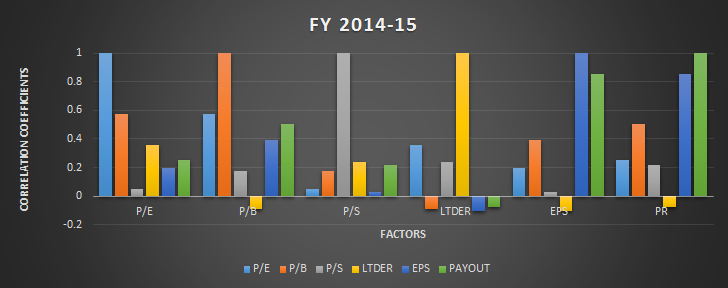
\includegraphics[width=3.5in ]{CC_2014-15}
	\caption{Dependencies of factors in FY 2014-15 }
	\label{fig2}
\end{figure}

\begin{figure}[!h]
	\centering
	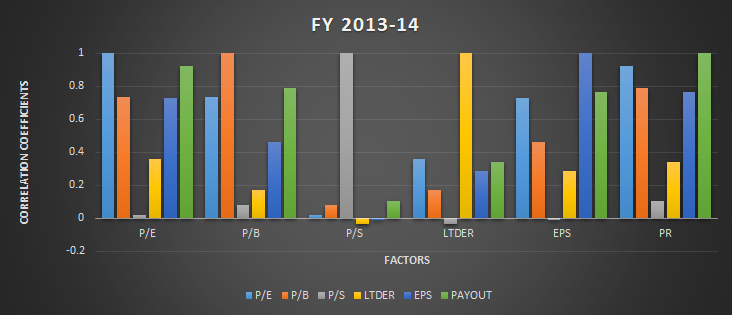
\includegraphics[width=3.5in ]{CC_2013-14}
	\caption{Dependencies of factors in FY 2013-14 }
	\label{fig3}
\end{figure}

\begin{figure}[!h]
	\centering
	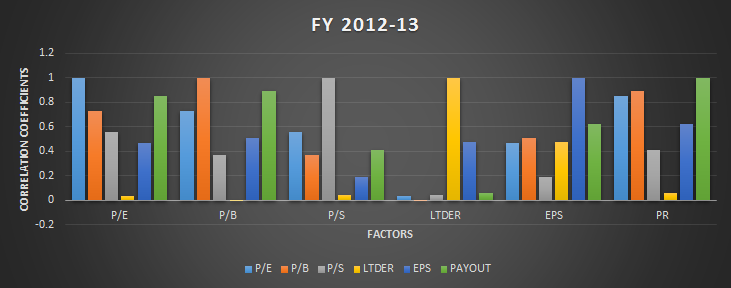
\includegraphics[width=3.5in ]{CC_2012-13}
	\caption{Dependencies of factors in FY 2012-13 }
	\label{fig4}
\end{figure}

In all the three years it is noticed that correlation coefficient values are high among P/E and P/B. This gives an 
indication that P/E and P/B are highly dependent with each other. EPS and PR are also found to be highly dependent. So 
if P/E and P/B are used as evidences in DS evidence theory at the same time, it may lead to a result of super estimate. 
The same is true for EPS and PR. But the dependencies of LTDER, P/S, P/E (or P/E) and EPS (or PR) among each other are 
relatively low. So all of these factors can be used as evidences for the DS synthesis of the proposed fuzzy rule based 
system. In this research finally the historical values of P/E, P/S, EPS and LTDER are treated as input to the proposed 
DS fuzzy expert system and are hence used for fuzzy rule construction and ranking of the 
stocks. 
\section{Brief introduction to DS evidence theory and fuzzy expert system}
DS evidence theory and fuzzy rule based expert system are hybridized in this work to 
evaluate and rank the stocks under BSE. Brief introduction of DS evidence theory and 
fuzzy rule based expert system are given here before their application in the proposed 
model is elaborated. 

\subsection{DS evidence theory}
A. P. Dempster in 1967 \cite{Dempster1967} proposed a multi-valued mapping from one space 
to another which was used for statistical inference when we needed to identify a single 
hypothesis from multiple sample information. The DS-theory was first proposed by Dempster 
in 1968 \cite{Dempster1968} and later in 1976 it was extended by Shafer 
\cite{Shafer1976} to deal with incomplete and uncertain information.

DS-Theory mainly deals with four components: Frame of discernment, Basic Probability 
Assignment (BPA), plausibility function \emph{Pl} and belief function \emph{Bel}. 

In evidence theory first a set of hypothesises $\Theta$ called frame of discernment, is assumed and defined as follows:
\begin{equation}
\Theta=\{H_1,H_2,H_3,...,H_N\}.
\end{equation} 
The set is composed of N mutually exhaustive and exclusive hypothesises. From the $\Theta$, let us denote $P(\Theta)$, 
be the power set composed with $2^N$ propositions $X$of $\Theta$:
\begin{equation}
P(\Theta)=\{\varnothing, \{H_1\}, \{H_2\},..., \{H_N\},\{H_1\cup H_2\}, \{H_1\cup H_3\},...,\Theta \}
\end{equation}  
where $\varnothing$ denotes the empty set. The most important task in applying evidence theory is Basic Probability 
Assignment (BPA). A BPA is a function from $P(\Theta)$ to $[0, 1]$ defined by:

\begin{equation}
\begin{aligned}
m:&  &P(\Theta)\rightarrow [0,1]\\
&  &X\mapsto m(A)
\end{aligned}
\end{equation}
and which satisfies the following criteria:
\begin{equation}
\begin{aligned}
\sum\limits_{X\in{P(\Theta)}}m(X)&=1;\\
m(\varnothing)&=1.
\end {aligned}
\end{equation}

Dempster's rule of combination is denoted by $m=m_1\oplus m_2$, which can combine two 
BPAs $m_1$ and $m_2$ to yield a new BPA:
\begin{equation}
\begin{aligned}
m(A)=\frac{\sum\limits_{Y\cap Z=A}m_1(Y)m_2(Z)}{1-k}
\end{aligned}
\end{equation}
with
\begin{equation}
\begin{aligned}
k=\sum\limits_{Y\cap Z=\varnothing}m_1(Y)m_2(Z)
\end{aligned}
\end{equation}
where k is a normalization constant, known as conflict because it measures the degree of 
conflict between $m_1$ and $m_2$. $k=0$ corresponds to the absence of conflict between 
$m_1$ and $m_2$, whereas $k=1$ implies total contradiction between them. The resulting 
belief function from the combination of $I$ information sources can be defined as:
\begin{equation}
m=m_1\oplus m_2 \oplus m_3 ... \oplus m_I
\end{equation} 

With the help of Equation (11) multi source information can be fused into a single 
framework in belief theory very easily and it proved to be very effective when it is 
applied in fuzzy rule generation discussed later in Section 3.3.3.

\subsection{Fuzzy Expert System}
For many real world problems, like strategic planning, medical diagnosis and other 
decision making problems solutions are something more than simple reasoning and require 
some expertise knowledge to solve. So the use of Expert Systems (ES) became popular 
because it is capable of representing and reasoning knowledge rich domain with a view to 
solve problems and giving advice \cite{jackson1986introduction}. The main advantage of ES 
over any other conventional software applications is its effective reasoning capability 
as they process knowledge instead of data or information 
\cite{darlington2000essence}. On the other hand the application of fuzzy set theory in 
uncertainty handling has become one of the strongest tool to design any framework. As 
fuzzy set theory is now widely applied in information  gathering,  modeling, analysis, 
optimization, control, decision-making and supervision \cite{bellman1970decision}, 
fuzzy expert system is used in the construction of the proposed model.

Fuzzy expert system is an expert system that uses fuzzy logic instead of Boolean logics 
in its knowledge base and derives conclusion from user inputs and fuzzy inference process 
\cite{kandel1991fuzzy}. Figure \ref{Fig5} depicts the basic architecture of a fuzzy 
expert system.

\begin{figure}[h]
	\centering
	\includegraphics[width=8cm,height=5.5cm]{architecture_FES}
	\caption{Architecture of Fuzzy Rule-based Expert System}
	\label{Fig5}
\end{figure} 

Various components of a fuzzy expert system are briefly discussed below:
\begin{itemize}
	
	\item \textbf{Fuzzy Knowledge Base}: Fuzzy knowledge base is a collection of fuzzy 
	rules and it is built up by the 	knowledge engineer after eliciting knowledge from 
	domain experts. The basic structure of a fuzzy rule is as follows:
	\begin{equation*}
	\text{IF } I_1 \text{ is } i_1 \text{ AND } I_2 \text{ is } i_2 \text{ AND ... AND } I_n \text{ is } i_n \text{ 
	THEN } O \text{ is }o. 
	\end{equation*}
	
	where $I_1$, $I_2$ ... , $I_n$ are fuzzy linguistic input variables and $i_1$, $i_2$, 
	... , $i_n$ are possible linguistic values of $I_1$, $I_2$ ... , $I_n$ respectively. 
	Similarly, $O$ is fuzzy linguistic output variable and 	$o$ is its linguistic value. 
	The terms $I_1$ is $i_1$ and $I_2$ is $i_2$ ... are fuzzy propositions suggesting  
	partial  set  membership  or  partial  truth. In this way modifying the fuzzy sets 
	parameters of the output fuzzy sets, the  partial  truth  of  the  rule premise can 
	be evaluated \cite{matthews2003formal}.
	
	\item \textbf{Fuzzy Inference Engine}: To  analyse  and manipulate  the  rules  in  
	the  knowledge  base an inference mechanism is adopted to conclude a logical result. 
	Various inference mechanisms  can  be  adopted  for  fuzzy  inference  engine  
	depending on  the  aggregation, implications and operators used for s-norms and 
	t-norms \cite{wang1999course}. Defuzzification of the results is also achieved  in 
	this module. This modules functions as per the agenda. An agenda is a prioritized 
	list of rules identified and enlisted by inference engine. Patterns of these rules 
	are satisfied by facts or objects in the working memory. 
	
	\item \textbf{Working Memory}: This module is contained of a global database of facts 
	those are going to be used by the fuzzy rule base.
	
	\item \textbf{Explanation Facility}: This particular module explains every steps in reasoning process of the ES.
	
	\item \textbf{Knowledge Acquisition Facility}: This module provides an automated facility for the user to enter 
	knowledge in the system.
	
	\item \textbf{User Interface}: All kinds of interactions of the user with the system is facilitated by this module. 
	This is used to accept inputs from the user and display the outcomes of the inference process.
\end{itemize}

%\subsection{Implementation of the Proposed Model}
%The designed diagram of the proposed model is introduced in Section 1 as Figure 
%\ref{fig:F1}. Here individual steps 
%followed to construct and implement the whole model are elaborated.

\section{Collection of historical data and its fuzzification}

Selection of input factors are discussed in details in section 4. Next stage of the 
development process is fuzzification of the historical data collected for these factors.

\subsection{Collection of historical data} 
Total 30 stocks are registered under BSE. Initially, historical data of last 12 years 
(2003-04 to 2014-15) of four factors (P/E, EPS, P/S and LTDER) are collected from 
different web sources like www.capitaline.com, www.bseindia.com, 
www.nseindia.com etc. First 9 years' data are used for the implementation of the model 
and last 3 years' data are used for testing and comparison. For the simplicity of the 
model the data are normalized within the range of [0, 10] by scaling up/down the maximum 
historical value of any factor in last 9 years to 10 and then scaling other data 
accordingly relative to the maximum value. Table 3 shows an example of actual and normalized data for Axis Bank Ltd.

\begin{table}[ht]
	\label{tab:Normalized_sample}
	\tbl{Sample normalized data for Axis Bank Ltd.}
	{\begin{tabular}{@{}ccc@{}} 
			\toprule
			Financial Year & Actual P/E ratio of Axis Bank Ltd. & Transferred Data \\
			\colrule
		2011-12	& 11.46	& 4.24 \\
		2010-11 &	17.5 &	6.48\\
		2009-10 &	19.47 &	7.2\\
		2008-09 &	8.49 &	3.14\\
		\bf 2007-08 &	\bf 27.02 &	\bf 10\\
		2006-07 &	21.67 &	8.02\\
		2005-06 &	21.12 &	7.82\\
		2004-05 &	20.5 &	7.59\\
		2003-04 &	12.54 &	4.64\\
		\botrule
		\end{tabular}}
	\end{table}

\subsection{Fuzzification}
Fuzzification is a process of taking a crisp value as input and transforming it into the 
degree required by the terms. Uncertainty basically comes from imprecision, vagueness or 
ambiguity and one of the best ways to represent these in any 
variable can be in the form of fuzzy variable. Fuzzy membership functions are used to represent the fuzzy variables. 
All four factors have been illustrated in Table 4 in terms of fuzzy linguistic variables and each of them has three 
linguistic values, \emph{Low, Standard and High}. Trapezoidal membership function has been used to represent the inputs 
within the range of [0, 10].

\begin{table}[h]
	\label{tab:MFs}
	\tbl{Membership functions for the linguistic values of the Input Variables}
	{\begin{tabular}{@{}ccc@{}} 
			\toprule
			Factors in terms of linguistic variables & Linguistic Values & Fuzzy Trapezoidal Membership\\
			\colrule
			\multirow {3}{3cm}{\centering P/E Ratio (Range 0 to 10)} & Low & (0 \hspace{0.12cm} 0 \hspace{0.12cm} 1.8 
			\hspace{0.12cm} 2.8) \\
			& Standard &(1.7 \hspace{0.12cm} 3.5 \hspace{0.12cm} 4.6 \hspace{0.12cm} 5.8)\\
			& High & (5.3 \hspace{0.12cm} 7.5 \hspace{0.12cm} 10 \hspace{0.12cm} 10)\\
			
			
		\multirow {3}{3cm}{\centering EPS (Range 0 to 10)} & Low & (0 \hspace{0.12cm} 0 \hspace{0.12cm} 2.2 
		\hspace{0.12cm} 
			3.5)\\ 
			& Standard &(2.5 \hspace{0.12cm} 4.6 \hspace{0.12cm} 5.6 \hspace{0.12cm} 7.9)\\ 
			& High & (6.4 \hspace{0.12cm} 9.6 \hspace{0.12cm} 10 \hspace{0.12cm} 10)\\ 
			
		\multirow {3}{3cm}{\centering P/S Ratio (Range 0 to 10)} & Low & (0 \hspace{0.12cm} 0 \hspace{0.12cm} 2.4 
		\hspace{0.12cm} 
			3.6)\\ 
			& Standard &(1.8 \hspace{0.12cm} 4.4 \hspace{0.12cm} 5.7 \hspace{0.12cm} 8.2)\\ 
			& High & (6.4 \hspace{0.12cm} 8.7 \hspace{0.12cm} 10 \hspace{0.12cm} 10)\\ 
						
		\multirow {3}{3cm}	{\centering LTDER (Range 0 to 10)} & Low & (0 \hspace{0.12cm} 0 \hspace{0.12cm} 2.3 
		\hspace{0.12cm} 3.6)\\ 
			& Standard &(2.8 \hspace{0.12cm} 4.6 \hspace{0.12cm} 5.7 \hspace{0.12cm} 7.6)\\ 
			& High & (6.124 \hspace{0.12cm} 8.09 \hspace{0.12cm} 10 \hspace{0.12cm} 10)\\ 
						
			\botrule
	\end{tabular}}
\end{table}


\section{Fuzzy Rule Construction using DS-Theory}
The most significant novelty of this research work is the application of DS evidence 
theory in fuzzy rule construction. The knowledge base of any fuzzy inference system is 
developed using collection of fuzzy rules which determines how the output will be 
generated based on the given input. The proposed system has four input parameters namely, 
P/E, EPS, P/S and LTDER, and based on these input parameter the DS-Fuzzy system is 
expected to determine whether the selection of any stock will be \emph{Highly Favourable, 
Moderately Favourable or Not Favourable}, as output. The frame of discernment is 
considered as $\Theta=\{\text {\emph{High Performance}}, \text{\emph { Average Performance}}, \text{\emph { and Poor 
Performance}}\}$. 

Risk/Return ratio is one of the most commonly used measure to evaluate the performance of stocks. Risk is generally 
measured by semi-variance(S) of the stocks' previous returns and Return(R) is actually the mathematical mean of 
previous returns. Obviously lower value of this ratio indicate better performance of stocks. Based on linguistic values 
of each input factors and comparing those with S/R values as a measure of the performance of various stocks BPAs for 
different hypothesises are achieved. The historical data of FY 2012-13 are used to identify the stocks. Consulting 
various domain experts and analysing historical data initially standard values for each factors for all the stocks are 
decided. By analysing last 9 years' historical data it is found that when P/E ratio was around its standard value then 
$75\%$ of stocks under BSE performed better and S/R value was also found to be satisfactory. So a belief of 0.75 is 
assigned towards the hypothesis $\{\text{\emph{High Performance}}\}$ when the P/E ratio is near to its standard value. 
Again, when P/E value found to be much lower than its standard value, $65\%$ of total stocks under BSE performed 
average and S/R value also found to be average. So 0.6 degree of belief is assigned towards the hypothesis 
$\{\text{\emph{Average Performance}}\}$ when P/E ratio is lower than its standard value. Similarly, when the value of 
P/E ratio was much higher than the standard value then it was found that $70\%$ of stocks under BSE performed poor and 
S/R value was also very high. So 0.7 degree of belief is assigned towards the hypothesis $\{\text{\emph{Poor 
Performance}}\}$. In the same way initial believes or Basic Probabilities are assigned for all other factors as 
mentioned in Table 5.

\begin{table}[h]
	\label{tab:BPA}
	\tbl{Basic Probability Assignment}
	{\begin{tabular}{@{}ccccc@{}} 
			\toprule
		Factors & Linguistic Values &  High Performance  &  Average Performance  &  Poor Performance 
		\\
		& & (H\_P) & (A\_P) & (P\_P)\\
		
		\colrule
		
		\multirow {3}{1cm}{P/E}
		& Low & { } & 0.6 & { }\\ 
		& Standard & 0.75 & { } & { }\\ 
		& High & { } & { } & 0.7\\ 
		
		\multirow {3}{1cm}{EPS}
		& Low & { } & { } & {0.8}\\ 
		& Standard & { } & {0.6} & { }\\ 
		& High & {0.65} & { } & { }\\ 
		
		
		\multirow {3}{1cm}{P/S}
		& Low & { } & { } & {0.7}\\ 
		& Standard & { } & {0.65} & { }\\ 
		& High & {0.75} & { } & { }\\ 
	
		
		\multirow {3}{1.5cm}{LTDER}
		& Low & {0.6} & { } & { }\\ 
		& Standard & { } & {0.75} & { }\\ 
		& High & { } & { } & {0.65}\\ 
		
			\botrule
		\end{tabular}}
	\end{table}

Now to elaborate further let us consider the following four sample rules with their initial belief:
\begin{enumerate}
	\item IF P/E is \textbf{Low} THEN Performance will be \textbf{Average} ($m_1\left( A\_P\right) =0.6$).
	\item IF EPS is \textbf{Standard} THEN Performance will be \textbf{Average} ($m_2\left( A\_P\right) =0.6$).
	\item IF P/S is \textbf{High} THEN Performance will be \textbf{High} ($m_4\left( H\_P\right) =0.75$).
	\item IF LTDER is \textbf{High} THEN Performance will be \textbf{Poor} ($m_6\left( P\_P\right) =0.65$).
\end{enumerate}
The above four rules represent the belief towards the performance of stocks with respect to the values of four input 
factors as the presence of evidences. Now consider the IF part of Rule 1 and Rule 2 as the first two evidences and 
$m_1$ and $m_2$ as mass functions for them respectively.

Now from Rule 1, $m_1(A\_P)=0.6$ and $m_1(\Theta)=(1-0.6)=0.4$, where, $m_1(\Theta)$ represents the degree of belief in 
the rest of the hypotheses present in the hypothesis set. Similarly, from Rule 2, $m_2(A\_P)=0.6$ and 
$m2(\Theta)=(1-0.6)=0.4$. Now these two mass functions are combined using Dempster's rule of combination (Equation 9) 
to obtain a new function $m_3$ as mentioned in Table 6.

\begin{table}[h]
	\label{tab:MCF1}
	\tbl{Combination of mass considering first two evidences}
	{\begin{tabular}{@{}ccc@{}} 
			\toprule
			Combining $m_1$ and $m_2$ & $m_2(A\_P)=0.6$ & $m_2(\Theta)=0.4$\\
			\colrule
			$m_1(A\_P)=0.6$ & $A\_P=0.36$ & $ A\_P=0.24$\\
			$m_1(\Theta)=0.4$ & $A\_P=0.24$ & $\Theta=0.16$\\
			\botrule
		\end{tabular}}
	\end{table}
	
The new mass value $m_3$ for the same hypothesis set is calculated as:
\begin{equation}
\begin{aligned}
\left. \begin{array}{ll}
\vspace{0.25cm}
m_3 (A\_P)&={0.36+0.24+0.24}=0.84\\
\vspace{0.25cm}
m_3(\Theta)&=0.16
\end{array}\right\}
\end {aligned}
\end{equation}

Now consider the IF part of the Rule 3 as the new evidence and $m_4$ be the new mass function. From Rule 3, 
$m_4(H\_P)=0.75$ and $m_4(\Theta)=(1-0.75)=0.25$. Now again, $m_3$ and $m_4$ are combined to generate new mass $m_5$ as 
mentioned in Table 7. 

\begin{table}[h]
	\label{tab:MCF2}
	\tbl{Combination of mass considering first three evidences}
	{\begin{tabular}{@{}ccc@{}} 
			\toprule
		Combining $m_3$ and $m_4$ & $m_4(H\_P)=0.75$ & $m_4(\Theta)=0.25$\\
			\colrule
			$m_3(A\_P)=0.84$ & $\Phi=0.63$ & $A\_P=0.21$\\
			$m_3(\Theta)=0.16$ & $H\_P=0.12$ & $\Theta=0.04$\\
			\botrule
		\end{tabular}}
	\end{table}

New mass values $m_5$ for the hypothesis set are calculated as below:
\begin{equation}
\begin{aligned}
\left. \begin{array}{ll}
\vspace{0.25cm}
m_5 (A\_P)&=\frac{0.21}{1-0.63}=0.567\\
\vspace{0.25cm}
m_5(H\_P)&=\frac{0.12}{1-0.63}=0.324\\
m_5(\Theta)&=\frac{0.04}{1-0.63}=0.108
\end{array}\right\}
\end {aligned}
\end{equation} 

Now if we consider the IF part of the Rule 4 as the last evidence and $m_6$ as its mass function then we get 
$m_6(H\_P)=0.6$ and $m_6(\Theta)=(1-0.6)=0.4$. Now finally, $m_5$ and $m_6$ are combined as mentioned in Table 8 to 
generate the final mass values $m_f$ for the hypothesis set (Equation 11).

\begin{table}[h]
	\label{tab:MCF3}
	\tbl{Combination of mass considering all four evidences}
	{\begin{tabular}{@{}ccc@{}} 
			\toprule
			Combining $m_5$ and $m_6$ & $m_6(P\_P)=0.65$ & $m_6(\Theta)=0.35$\\
			\colrule
			$m_5(A\_P)=0.567$ & $\Phi = 0.368$ & $A\_P=0.198$\\
		$m_5(H\_P)=0.324$ & $\Phi=0.21$ & $H\_P=0.113$\\
		$m_5(\Theta)=0.108$ & $P\_P=0.07$ & $\Theta=0.037$\\
			\botrule
		\end{tabular}}
	\end{table}
	
	
	\begin{equation}
	\begin{aligned}
	\left. \begin{array}{ll}
	\vspace{0.25cm}
	m_f (H\_P)&=\frac{0.113}{1-0.578}=0.267\\
	\vspace{0.25cm}
	m_f(A\_P)&=\frac{0.198}{1-0.578}=0.469\\
	\vspace{0.25cm}
	m_f(P\_P)&=\frac{0.07}{1-0.578}=0.165\\
	\vspace{0.25cm}
	m_f(\Theta)&=\frac{0.37}{1-0.578}=0.087
	\end{array}\right\}
	\end {aligned}
	\end{equation} 
	
Following the same procedure final mass values for the rest 80 rules are calculated. For the hypothesis \emph{High 
Performance(H\_P)} maximum and minimum mass values ($m_f$) are found to be $0.9916$ and $0$ respectively. As mass 
values for any hypothesis can lie between $0$ and $1$ we have divided the favourability of any stock, based on the 
$m_f(H\_P)$ of the rules, into three categories: \emph{Highly Favourable} $(0.76\leq m_f(H\_P)\leq 1)$, 
\emph{Moderately Favourable} $(0.46\leq m_f(H\_P)\leq 0.75)$ and \emph{Not Favourable} $(m_f(H\_P)\leq 0.45)$.

So the combined version of the four sample rules mentioned earlier is formed as:
``IF P/E is \textbf {Low} AND EPS is \textbf{Standard} AND P/S is \textbf {High} AND LTDER is \textbf {High} THEN the 
stock is \textbf{Not Favourable}".

In this way total 81 fuzzy rules are formulated using DS evidence theory to develop the knowledge base of the proposed 
DS-fuzzy inference system and the above mentioned three selection categories are converted into fuzzy linguistic 
variables with trapezoidal membership values as shown in Table 9 for output of the proposed inference 
system. 	

\begin{table}[h]
	\label{tab:MFOUTPUT}
	\tbl{Degree of membership of linguistic values for the output variable}
	{\begin{tabular}{@{}ccc@{}} 
			\toprule
		 Output Variable &  Linguistic Values &  Fuzzy Trapezoidal Membership\\
			\colrule
			\multirow {3}{3cm}{\centering Selection (Range: 0 to 1)} & Not Favourable & (0 \hspace{0.12cm} 0 
			\hspace{0.12cm} 0.172 \hspace{0.12cm} 0.448) \\
			& Moderately Favourable &(0.34 \hspace{0.12cm} 0.46 \hspace{0.12cm} 0.57 \hspace{0.12cm} 0.75)\\
			& Highly Favourable & (0.64 \hspace{0.12cm} 0.88 \hspace{0.12cm} 1 \hspace{0.12cm} 1)\\
			\botrule
		\end{tabular}}
	\end{table}

Figure \ref{fig:F3} shows the snapshot of the fuzzy rule base and Figure \ref{fig:F4} shows the sensitivity analysis 
of the same when designed in MATLAB. 
\begin{figure}[h]
	\centering
	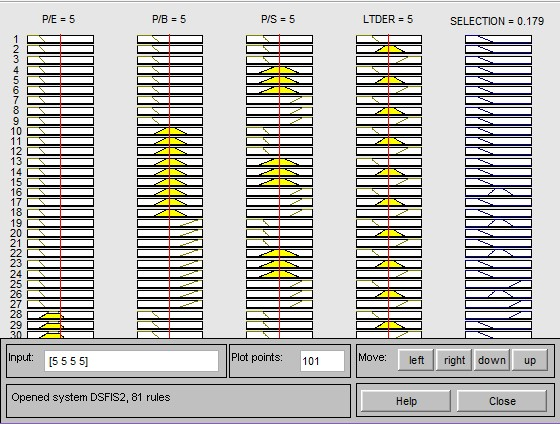
\includegraphics[width=9cm,height=6cm]{Rule_base}
	\caption{Fuzzy rule base of the DS-fuzzy system for Stock Selection}
	\label{fig:F3}
\end{figure}

\begin{figure}[h]
	\centering
	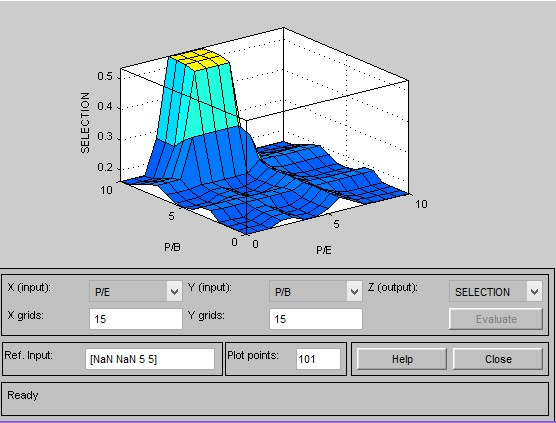
\includegraphics[width=9cm,height=6cm]{Sensitive_analysis}
	\caption{The Sensitivity analysis of the DS-fuzzy system for Stock Selection}
	\label{fig:F4}
\end{figure}

\section{Defuzzification and ranking of stocks}
The process of obtaining a single value that represent the best outcome of the fuzzy set evaluation is known as 
defuzzification \cite{Ngai2003}. Though there are many other popular defuzzification methods namely, Bi-sector, Mean of 
Maximum (MOM), Smallest of Maximum (SOM), Largest of Maximum (LOM), in this proposed model `Centroid' is used for the 
defuzzification purpose due to its wide range of acceptability. This method was introduced by Sugeno in 1985 and it can 
be expressed as:

\begin{equation}
\begin{aligned}
z^*=\frac{\int \mu_{\utilde{C}}(z)\cdot zdz}{\int \mu_{\utilde{C}}(z)dz}
\end{aligned}
\end{equation}

Where  $z$ is the output variable, $z^*$ is the defuzzified output value and $\mu_{\utilde{C}}(z)$ is the aggregated 
membership function.

The proposed DS-fuzzy system is used to rank all 30 registered stocks under BSE based on 
the defuzzified outputs when the values corresponding to each of the four input factors 
for 2012-13 for each stocks are provided as input to the system. Top 10 stocks from this 
ranking are mentioned in Table 10. 

\begin{table}[h]
	\label{tab:Top_Stocks}
	\tbl{Top 10 Stocks based on the input data for FY 2012-13}
	{\begin{tabular}{@{}ccc@{}} 
			\toprule
			 Sl. No &  Name of the Stocks & Defuzzified Values(FY 2012-13)\\
			\colrule
			{1} & {Hindustan Unilever Ltd.} & {0.8644}\\
			
			{2} & {Sun Pharmaceutical Inds. Ltd.} & {0.8457}\\
		
			{3} & {ITC Ltd.} & {0.5369}\\
			
			{4} & {Coal India Ltd.} & {0.534}\\
			
			{5} & {Tata Consultancy Services Ltd.} & {0.4936}\\
			
			{6} & {Infosys Ltd.} & {0.3842}\\
			
			{7} & {Dr. Reddy's Laboratories Ltd.} & {0.3553}\\
			
			{8} & {Bajaj Auto Ltd.} & {0.3292}\\
			
			{9} & {Hero Motocorp Ltd.} & {0.3002}\\
			
			{10} & {Cipla Ltd.} & {0.285}\\
			
			\botrule
		\end{tabular}}
	\end{table}

As the consequent of every rule indicates the favourability of the stocks, higher defuzzified value indicate higher 
favorability. The highest defuzzified value of $0.8691$ is found for \emph{Hindustan Unilever Ltd.} among all 30 
registered stocks and it has topped the ranking. These 10 stocks are used for portfolio construction as discussed in 
the next section.

\section{Portfolio Construction}
The first phase of stock portfolio selection, i.e. the selection of suitable stocks, is 
achieved in the previous section. In this section a portfolio construction model is 
discussed to determine optimum investment ratios for the selected securities such that 
the overall return is maximized under a tolerable risk. 

\subsection{Objective Function}
The ratio of the difference of fuzzy portfolio return and the risk free return to weighted mean semi-variance of the 
assets is used as the objective function in this work. Certainly, higher value of this ratio will indicate the better 
investment; so the optimization target will be to maximize the ratio.

The notations used for the construction of this objective function are mentioned below:
\begin{itemize}
	\item $x_i$: Fraction of the total investment allotted to the $i^{th}$ asset;
	\item $\tilde{r_i}$: Fuzzy return of the $i^{th}$ asset;
	\item $r_f$: Risk free return rate;
	\item $\mu_s$: Weighted mean of asset semi-variances;
	\item $r_p$: Portfolio return;
	\item $v_p$: Variance of the portfolio;
	\item $s_p$: Skewness of the portfolio;
\end{itemize} 
Thus the objective function is formed as:
\begin{equation}
\begin{aligned}
Maximize \frac{E(\sum \tilde{r_i}x_i)-r_f}{\mu_s}
\end{aligned}
\end{equation} 
Where, after descending sort of portfolio, $\mu_s=\sum x_i s_i$, i.e. $x_i$ is the $i^{th}$ weight in the descending 
order and $s_i$ is the semi-variance of the $i^{th}$ ranked asset.

A fuzzy aggregation is used to calculate the fuzzy returns of the securities from the statistical database of past five 
years(2008-09 to 2012-13). If $t_i$ means $i^{th}$ position of the data, the fuzzy return can be calculated as:
\begin{equation}
\begin{aligned}
\tilde{r_i}=\left( { min(r_i),\frac{\sum t_i r_i}{\sum t_i},max(r_i)}\right) 
\end{aligned}
\end{equation}

The constraints included in this model are:

\begin{equation}
\begin{aligned}
\left. \begin{array}{ll}
\vspace{0.25cm}
r_p>\alpha, v_p>\beta, s_p>\gamma\\
\sum\limits_{i=1}^{n}x_i=1, x_i\leq M, x_i>0, \forall i
\end{array}\right\}
\end {aligned}
\end{equation}
Values for $\alpha$,$\beta$, $\gamma$, $M$ and $m$ are decided based on the investor's preferences. 

Thus the final portfolio optimization model can be summarized as below:
\begin{equation}
\begin{aligned}
\left. \begin{array}{ll}
\vspace{0.25cm}
Maximize \frac{E(\sum \tilde{r_i}x_i)-r_f}{\mu_s}\\
\text{Subject to, }\\
\vspace{0.25cm}
r_p>\alpha, v_p>\beta, s_p>\gamma\\
\vspace{0.5cm}
\sum\limits_{i=1}^{n}x_i=1, x_i\leq M, x_i>0, \forall i
\end{array}\right\}
\end {aligned}
\end{equation}

\subsection{Optimization of the proposed model using ACO}
An algorithm using Ant Colony Optimization (ACO) is proposed and implemented in this section to solve the optimization 
model as mentioned in Equation (19). ACO is a very popular meta-heuristic optimization technique inspired by the 
foraging behaviour of biological ants \cite{Dorigo2006,Deneubourg1990}. Pseudo code of the proposed algorithm is given 
as below:

\begin{algorithm}
	\caption{ACO algorithm for portfolio optimization}
	\label{ACOportfolio}
	\begin{algorithmic}[1]
		\Procedure {ACO-Portfolio}{}
		\State Generate N random solution nodes based on Equation (19);
		\State Initialization of the ACO;
		\For {ITERATION=1 to I}
		\For {ANT=1 to $\Gamma$}
		\State Select the start node randomly;
		\For {LIFETIME=2 to L}
		\State \begin{varwidth}[t]{10cm}
			Select the next node based on the heuristic information and pheromone concentration in the path. Move to 
			the next node only if it is better than the current node;\\
		\end{varwidth}
		\State Update pheromone on the selected path;
		\EndFor
		\State Store the details of the final node reached by each ants;
		\EndFor
		\State 
		\begin{varwidth}[t]{10.5cm}
			Identify the solution node where maximum number of ants reached and consider that to be the optimum 
			solution for the current solution;\\
		\end{varwidth} 
		
		\State 
		\begin{varwidth}[t]{10.75cm}
			Update the pheromone on the path of each ants who have reached this optimum solution;\\
		\end{varwidth}
		\State Evaporate the pheromone from all paths.
		\EndFor
		
		\EndProcedure
	\end{algorithmic}
\end{algorithm}

To execute the above algorithm in this work, initially 2000 random solutions are generated for the ant colony of 50 
ants. Total 400 iterations are used for the optimization purpose while lifetime for each ant is considered as 20. 

In Equation (19), $\tilde{r_i}$ is represented as a triangular fuzzy number. The Expected Return (E), Variance (Var), 
Skewness (Skew) and Semi-variances of these top 10 securities for past five years (2008-09 to 2012-13) as used in the 
above algorithm are calculated by the following theorem and are mentioned in Table 11.

%\newtheorem{theorem}{Theorem}[section]
\begin{theorem}
	Let $\tilde{A}=(a,b,c)$ be a triangular fuzzy number. The  the weighted possibilistic mean, variance and skewness 
	can be calculated as \cite{Bhattacharyya2013}:
	\begin{equation}
	\begin{aligned}
	\left. \begin{array}{ll}
	\vspace{0.25cm}
	E(\tilde{A})&=\frac{1}{6}(a+4b+c)\\
	\vspace{0.25cm}
	Var(\tilde{A})&=\frac{1}{18}(a^2+b^2+c^2-ab-bc-ca)\\
	\vspace{0.25cm}
	Skew(\tilde{A})&=\frac{19(a^3+c^3)-8b^3-42b(a^2+c^2)+12b^2(a+c)-15(a^2c+ac^2)+60abc}{10\sqrt{2}(\sqrt{a^2+b^2+c^2-ab-bc-ca})^3}
	\end{array}\right\}
	\end {aligned}
	\end{equation}
\end{theorem}  

\begin{table}[h]
	\label{tab:ER_V_Sk_S}
	\tbl{Expected Return, Variance, Skewness and Semivariance of stocks}
	{\begin{tabular}{@{}cccccc@{}} 
			\toprule
			Rank &  Name of the Stocks &  Return &  Variance &  Skewness &  Semivariance\\
			\colrule
			{1}& {Hindustan Unilever Ltd.} & {0.1443} & {0.0001} & {0.2391}  & {0.00004}\\
			{2} & {Sun Pharmaceutical Inds. Ltd.}& {0.0529} & {0.0006} & {-0.3269} & {0.00254}\\
			{3} & {I T C Ltd.} & {0.2801} & {0.0035} & {0.7523} & {0.00314}\\
			{4} & {Coal India Ltd.} & {0.1275} & {0.0028} & {0.6046} & {0.0373}\\
			{5} & {Tata Consultancy Services Ltd.} & {0.1228} & {0.0013} & {-0.5029} & {0.00557}\\
			{6} & {Infosys Ltd.} & {0.0356} & {0.0003} & {0.8648} & {0.0002}\\
			{7} & {Dr. Reddy'S Laboratories Ltd.} & {0.0484} & {0.0006} & {-0.0065} & {0.00098}\\
			{8} & {Bajaj Auto Ltd.} & {0.0579} & {0.001} & {0.7262} & {0.0013}\\	
			{9} & {Hero Motocorp Ltd.} & {0.1379} & {0.0004} & {0.8057} & {0.00049}\\
			{10} & {Cipla Ltd.} & {0.0437} & {0.0002} & {0.8258} & {0.00018}\\
			\botrule
		\end{tabular}}
	\end{table}
	
When the algorithm is executed in MATLAB with the above dataset and considering other parameters as $r_f=0.01$, $ \beta 
=0.5 $, $\alpha =0.05$, $ \gamma =0.001$, $ M=0.8 $ and $ \mu_s=0.0016 $, the maximum return is found as $0.1317$. The 
proposed ratio allocation for this return is given in Table 12.

\begin{table}[h]
	\tiny
	\label{tab:Ratio_allocation}
	\tbl{Ratio allocation for the proposed portfolio}
	{\begin{tabular}{@{}cccccccccc@{}} 
			\toprule
				Hindustan & Sun  & ITC  & Coal  & TCS  & Infosys & 
				Dr.   & Bajaj & Hero  & Cipla  \\
				
				Unilever  &  Pharma. & Ltd. & India  & Ltd. &  Ltd. & Reddy's &  Auto  & Motocorp 
			& Ltd.\\
				
				Ltd. & Inds. Ltd.& & Ltd.& &  & Lab. Ltd. & Ltd. & Ltd. &  \\
				
			\colrule
			0.2403 & 0.2235 & 0.1970 & 0.0764 & 0.0574 & 0.0525 & 0.0452 & 0.0413 & 0.0407 & 0.0255 \\
			\botrule
		\end{tabular}}
	
	\end{table}
	
	The convergence of the objective values as per the proposed model is depicted in Figure \ref{fig:F5} and the 
	accumulation of ants to the optimum objective values in each iteration is depicted in Figure \ref{fig:F6}. 
	
	\begin{figure}[h]
		\centering
		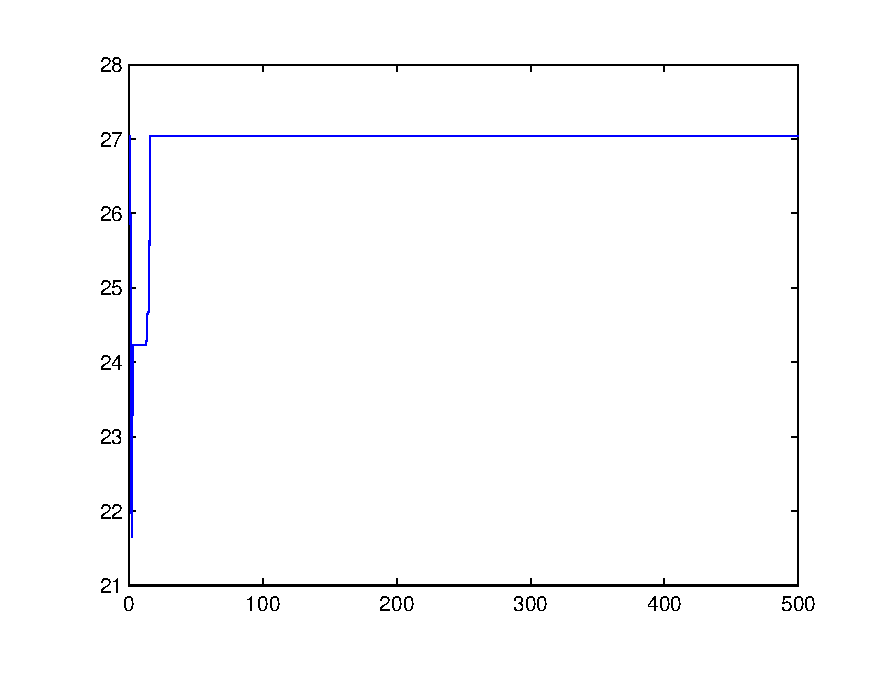
\includegraphics[width=9cm,height=6cm]{F5}
		\caption{Convergence of objective values based on proposed ranking}
		\label{fig:F5}
	\end{figure}
	
	\begin{figure}[h]
		\centering
		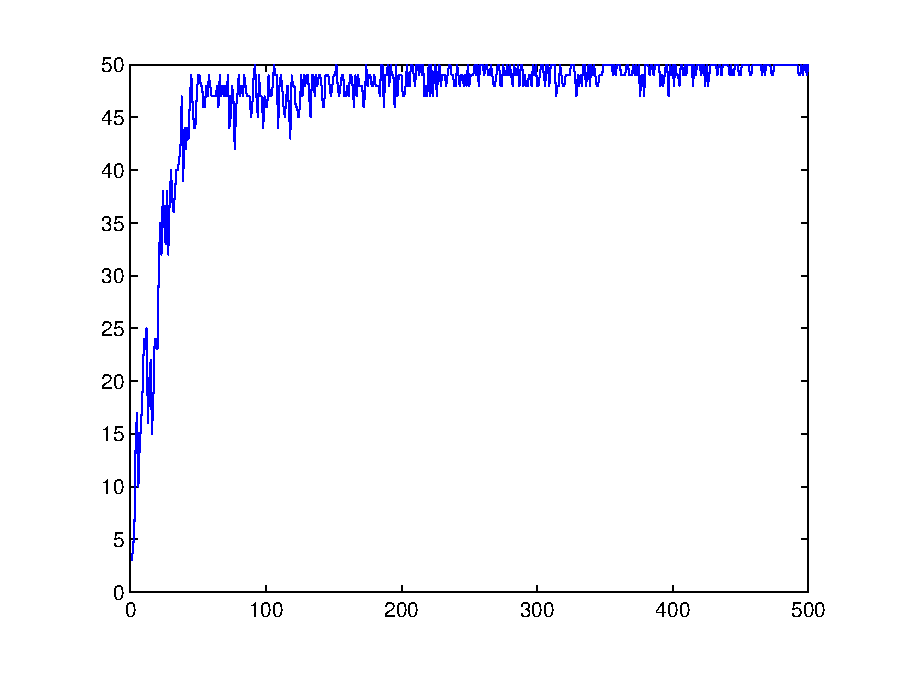
\includegraphics[width=9cm,height=6cm]{ant_acu}
		\caption{Ant accumulation at optimum solutions}
		\label{fig:F6}
	\end{figure} 
	
	\section{Result Analysis}
In this section we have analyzed the performance of our proposed model in three different aspects. 

\subsection{Adaptability of the proposed model}
Initially a ranking based on the S/R values of the stocks for the year 2012-13 is prepared and then a portfolio with 
top 10 stock from this ranking is constructed using the same objective value and ACO  algorithm.

Figure \ref{fig9} shows how the objective values are converged and Figure \ref{fig10} displays the accumulation of ants 
at optimum nodes in each iterations.    

\begin{figure}[!h]
	\centering
	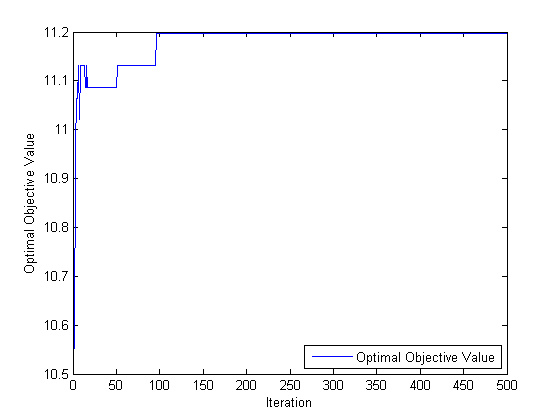
\includegraphics[width=3.5in]{Optimization_SR}
	\caption{Convergence of objective values}
	\label{fig9}
\end{figure}

\begin{figure}[!h]
	\centering
	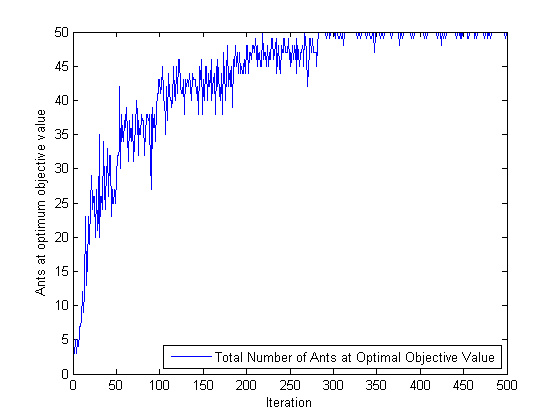
\includegraphics[width=3.5in]{Ant_Accu-SR}
	\caption{Ant accumulations at optimum solutions}
	\label{fig10}
\end{figure}

Return and risk of these two portfolios are compared in Table 13 and graphical representation of this comparison is 
shown in Figure 

\begin{table}[h]
	\centering
	\tiny
	\label{tab:Proposed_Vs_S/R}
	\tbl{Ratio allocation for the proposed portfolio}
	{\begin{tabular}{@{}cccc@{}} 
			\toprule
			Type of the  & Portfolio Return  & Portfolio 
			Risk  & Risk-Return  \\
			portfolio & ($\sum \tilde{R_i}x_i$) & ($\mu_s$) & Ratio \\
			\colrule
	
		Based on proposed ranking & 0.1316 & 0.0044 & 0.0334\\
	
		Based on ranking using S/R values & 0.0740 & 0.0057 & 0.0772\\
		
			\botrule
		\end{tabular}}
		
	\end{table}	
	
	 \begin{figure}[!h]
	 	\centering
	 	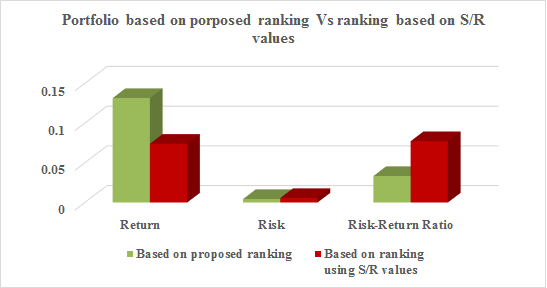
\includegraphics[width=3.5in]{Proposed-vs-SR}
	 	\caption{Portfolio based on proposed ranking and based on ranking using S/R values}
	 	\label{fig11}
	 \end{figure}
	
	It is noticed that portfolio constructed based on the proposed ranking is capable of giving better return under 
	comparatively lower risk. This outcome assures the adaptability of the proposed model by ensuring better portfolio 
	return for short term investment period.
	
	\subsection{Stability and effectiveness of the proposed model}
	To check the reliability of the proposed ranking data are collected for next three financial years (FY 2013-14, FY 
	2014-15, FY 2015-16) and then stocks are ranked in risk-return framework. When these ranking are compared with the 
	predicted top 15 stocks using the proposed model a match for 10, 11 and 9 companies are found in FY 2013-14, FY 
	2014-15 and FY 2015-16 respectively.
		
\begin{table}[!h]
	\tiny
	\caption{Top 15 stocks under BSE}
	\begin{center}
		\label{tab:Rank_Comparison}
		\begin{tabular}{  >{\centering\arraybackslash}m{0.2in}  
				>{\centering\arraybackslash}m{0.70in} 
				>{\centering\arraybackslash}m{0.70in}>{\centering\arraybackslash}m{0.2in} 
				>{\centering\arraybackslash}m{0.70in}
				>{\centering\arraybackslash}m{0.2in} >{\centering\arraybackslash}m{0.70in}
				>{\centering\arraybackslash}m{0.2in}}
		\toprule
			Rank & Top 15 based the proposed model & Top 15 based on performance (2013-14) & S/R  &	Top 15 based on 
			performance (2014-15) &	S/R &	Top 15 based on performance (2015-16) &	S/R \\
		\vspace{0.25cm}\\
		\colrule
		\vspace{0.5cm}\\
			1 & Hindustan Unilever Ltd. & Hero Motocorp Ltd. & 0.035 & ITC Ltd. & 0.019& TCS Ltd.& 0.034	\\
		\vspace{0.5cm} \\
			
			2 & Sun Pharmaceutical Inds. & ITC Ltd. & 0.043& HDFC Bank Ltd. & 0.062&ITC Ltd. & 0.042\\
		\vspace{0.5cm} \\		
			
			3 & ITC Ltd. & Hindustan Unilever Ltd. & 0.081& Hero Moto Corp Ltd. & 0.116& Hindustan Unilever Ltd.& 
			0.056\\
		\vspace{0.5cm} \\	
			
			4 & Coal India Ltd. & Hindalco Industries Ltd. & 0.087 & Hindustan Unilever Ltd. & 0.122& Tata Power Co. 
			Ltd. & 0.064\\
		\vspace{0.5cm} \\
			
			5 & TCS Ltd. & HDFC Ltd. & 0.123 & Wipro Ltd. &0.142 &State Bank Of India & 0.114	\\
		\vspace{0.5cm} \\	
			
			6 & Infosys Ltd. & TCS Ltd. & 0.130& Maruti Suzuki India Ltd. & 0.162& HDFC Bank Ltd.& 0.117	\\
		\vspace{0.5cm} \\
			
			7 & Dr. Reddy's Laboratories Ltd. &	HDFC Bank Ltd. &0.146 & Tata Power Co. Ltd. &0.167 & Wipro Ltd. & 
			0.140\\
		\vspace{0.5cm} \\	
			
			8 & Bajaj Auto Ltd. &	Tata Power Co. Ltd.& 0.166 & Tata Motors Ltd.& 0.177& ICICI Bank Ltd. & 
			0.191\\
		\vspace{0.5cm} \\	
			
			9 & Hero Moto Corp Ltd. & Coal India Ltd.& 0.180& TCS Ltd.& 0.181& Coal India Ltd. & 0.218	\\
		\vspace{0.5cm} \\		
			
			10 & Cipla Ltd. & Dr. Reddy's Laboratories Ltd.& 0.234& Coal India Ltd.&0.182 & Larsen \& Toubro 
			Ltd. & 0.256	\\
		\vspace{0.5cm} \\
			
			11 & HDFC Bank Ltd.	& Mahindra \& Mahindra Ltd.&0.237 & Mahindra \& Mahindra Ltd.&0.188 & HDFC Ltd.& 0.287 
			\\
		\vspace{0.5cm} \\
			
			12 &  Wipro Ltd. & Tata Motors Ltd.&0.242 & Cipla Ltd. & 0.188& Sun Pharmaceutical Inds. Ltd. & 
			0.335\\
		\vspace{0.5cm} \\	
			
			13 & Larsen \& Toubro Ltd.  & Cipla Ltd. &0.262 & Sun Pharmaceutical Inds. Ltd.& 0.246& Vedanta 
			Limited & 0.436\\
		\vspace{0.5cm} \\
			
			14 & Bharti Airtel Ltd. & Bajaj Auto Ltd. & 0.272& NTPC Ltd. & 0.271& Mahindra \& Mahindra Ltd. & 0.540\\
		\vspace{0.5cm} \\
			
			15 & Tata Power Co. Ltd. & Bharat Heavy Electricals Ltd. & 0.305& Bharti Airtel Ltd. &0.274 & Hindalco 
			Industries Ltd. &0.635 \\
			\vspace{0.25cm}\\
		\botrule
					
		\end{tabular}	
	\end{center}
\end{table}

Presence of similar stocks in the above rankings promotes the effectiveness and stability of the proposed model for 
short and mid term investment periods. 

\subsection{Comparison of other existing expert systems with the proposed model- An empirical 
study}
In dynamic uncertain environment selection of suitable stocks from any stock market for portfolio construction is 
always an challenging issue. In section 1 we have mentioned few researches which have addressed this challenging issue. 
In this article we propose a DS theory based fuzzy expert system to address the challenges of stock selection and 
portfolio construction. In literature we found four experts systems prior to these this work to address these 
challenging issues. These expert systems are implemented in different stock exchanges using different input factors and 
different fuzzy inference engines. So, we compared our proposed model with these four expert systems empirically. Table 
\ref{tab:performance_comparison} shows details of these comparison. 

\begin{table}[!h]
	\tiny
	\caption{Empirical comparison of other ES with the proposed ES model}
	\begin{center}
		\label{tab:performance_comparison}
		\begin{tabular}{ >{\centering\arraybackslash}m{0.25in}  
				>{\centering\arraybackslash}m{0.75in} >{\centering\arraybackslash}m{0.25in} 
				>{\centering\arraybackslash}m{0.65in} >{\centering\arraybackslash}m{0.5in}
				>{\centering\arraybackslash}m{0.75in} 
				>{\centering\arraybackslash}m{0.5in}}
			\toprule
			
			Article & Factors identified for the ES & Rule base size & 
			Portfolio construction & Optimization Tool used & Results analysis and tested data source & Uncertainty 
			handling tool \\
			\vspace{0.25cm}\\
			\colrule
			\vspace{0.5cm} \\
					
			\cite{Dymova2010new} & Different types of price and volume changes are used as parameters & 108 & Not 
			Address & 
			NA & Tested on real data from Warsaw Stock Exchange & Fuzzy sets and DS evidence theory\\
				\vspace{0.5cm} \\
				
			\cite{Xidonas2009} & Criteria based on fundamental analysis technique for making rational investment 
			decision 
			within long term period & 1406 & Not Address & NA & firms whose equities are traded in Athens Stock 
			Exchange 
			leveraging from the expert opinions & No well-known tool is used \\
			\vspace{0.5cm} \\
			
			\cite{Yunusoglu2013fuzzy} & 15 fundamental and 5 technical data are used as input to the ES & 81 & A model 
			is constructed to maximize the total weighted ratings of the stocks incorporated in the recommended 
			portfolio & Mixed integer linear programming model & Tested on real data from Istanbul Stock Exchange & 
			Fuzzy sets \\
			\vspace{0.5cm} \\
			
			\cite{Fasanghari2010design} & Seven factors are identified specified by experts mainly focusing on 
			technical criteria & 932 & Based on different investment criteria provided by investors through 
			questionnaires & No optimization tool is used & Tested on real data from Tehran Stock Exchange & Fuzzy Sets 
			\\
				\vspace{0.5cm} \\
			
			This article & 4 fundamental factors identified based on experts' consensus   & 81	& A 
			model is used to maximize the difference of fuzzy portfolio	return and the risk free return to the weighted
			mean semi-variance of the assets & ACO & Tested on real data from Bombay Stock Exchange & Fuzzy Sets and 
			DS evidence theory \\
				\vspace{0.25cm}\\	
				\botrule
		\end{tabular}
	\end{center}
\end{table} 

Fuzzy rule base of previous expert systems were mainly designed based on experts' opinions. This may significantly 
increase the development time and cost as the size of the rule base increases. These constraints are overcome 
significantly in this model as DS evidence theory is used here to generate automated fuzzy rule base. Inherent 
uncertainty in the design of the fuzzy rule base is also addressed at the same time.

Robustness of the proposed portfolio optimization model is another advantage. As performance of stocks are uncertain 
and dynamic in nature use of fuzzy return and and risk with fuzzy variance and skewness has considerably increased the 
robustness of the system.

All these improvements demonstrate the superiority of the proposed model over other existing expert systems.

\section{Conclusion}
\noindent In this research a novel fuzzy expert system model is designed and implemented to evaluate and rank the 
stocks under BSE. DS-evidence theory is used for the development of the fuzzy rule base to reduce the overall 
implementation time and cost of the system. A portfolio optimization model is constructed by considering the ratio of 
the difference of fuzzy portfolio return and risk free return to the weighted mean semi-variance of the assets as the 
objective function. ACO is used to obtain the optimum value of this portfolio. 

As the outcome of this model found to be satisfactory, this can be implemented for any stock exchanges around the world 
but the selection of critical factors may vary over different stock exchanges. This fuzzy expert system model can be 
used to rank any set of alternatives based on the factors influencing them. The portfolio optimization model and the  
related ACO algorithm can be used to optimize any rank-preference based portfolios. 

This work can be extended to include analysis of expert system on integrated data of assets from different stock 
exchanges and mutual funds. In this work ACO is used for optimization purpose. Researchers can use some other 
meta-heuristic algorithms such as  simulated annealing, tabu search, particle swam optimization, genetic algorithm to 
find the portfolio.  

\section*{References}

\bibliographystyle{elsarticle-num}
\bibliography{BIBPORTFOLIO}
\end{document}
